\section{Probability Ensembles and Exploratory Matched-Generator Adaptation}
\label{app:ensemble}

\subsection{Panel~A Probability-Mean Ensembles (Zero Retraining)}

Using the frozen per-sample prediction assets, we form \textbf{equal-weight probability-mean} ensembles without retraining, without UFD-based member selection, and without any test-set weight tuning (fixed equal weights only).
Table~\ref{tab:ensemble} compares singles to four ensembles: all six Panel~A models; LiteSSM-A with EfficientNet-B0; the top-three ID/UFD members (LiteSSM-A/B + EfficientNet-B0); and the SSM pair.
Figure~\ref{fig:ensemble} visualizes UFD Macro.
The regeneration script is \texttt{scripts/run\_ensemble\_panel\_a.py}.

\begin{table}[H]
\caption{Panel~A singles versus equal-weight probability-mean ensembles from frozen predictions (no retraining; no test-set weight tuning; fixed members).
UFD Macro remains the primary cross-generator summary; ensembles were not used to alter the preferred operating point.\label{tab:ensemble}}
\scriptsize
\setlength{\tabcolsep}{3.5pt}
\begin{tabularx}{\textwidth}{@{}L*{4}{R}@{}}
\toprule
\textbf{Model / Ensemble} & \textbf{ID AUC} & \textbf{UFD Macro} & \textbf{Worst} & \textbf{DALL·E} \\
\midrule
LiteSSM-A & 0.946 & \textbf{0.718} & 0.504 & 0.504 \\
LiteSSM-B & 0.945 & 0.700 & 0.484 & 0.484 \\
EfficientNet-B0 & 0.929 & 0.667 & 0.519 & 0.519 \\
LiteFreqNet~v2 & 0.906 & 0.645 & 0.451 & 0.451 \\
MobileNetV3-S & 0.890 & 0.636 & 0.455 & 0.455 \\
ShuffleNet-x0.5 & 0.880 & 0.674 & 0.467 & 0.467 \\
\midrule
$E_{\mathrm{all6}}$ mean & 0.943 & 0.703 & 0.471 & 0.471 \\
$E_{\mathrm{A+Eff}}$ mean & 0.945 & 0.709 & 0.524 & 0.524 \\
$E_{\mathrm{top3}}$ mean & 0.950 & 0.712 & 0.511 & 0.511 \\
$E_{\mathrm{A+B}}$ mean & 0.948 & 0.713 & 0.495 & 0.495 \\
\bottomrule
\end{tabularx}
\end{table}

\begin{figure}[H]
\centering
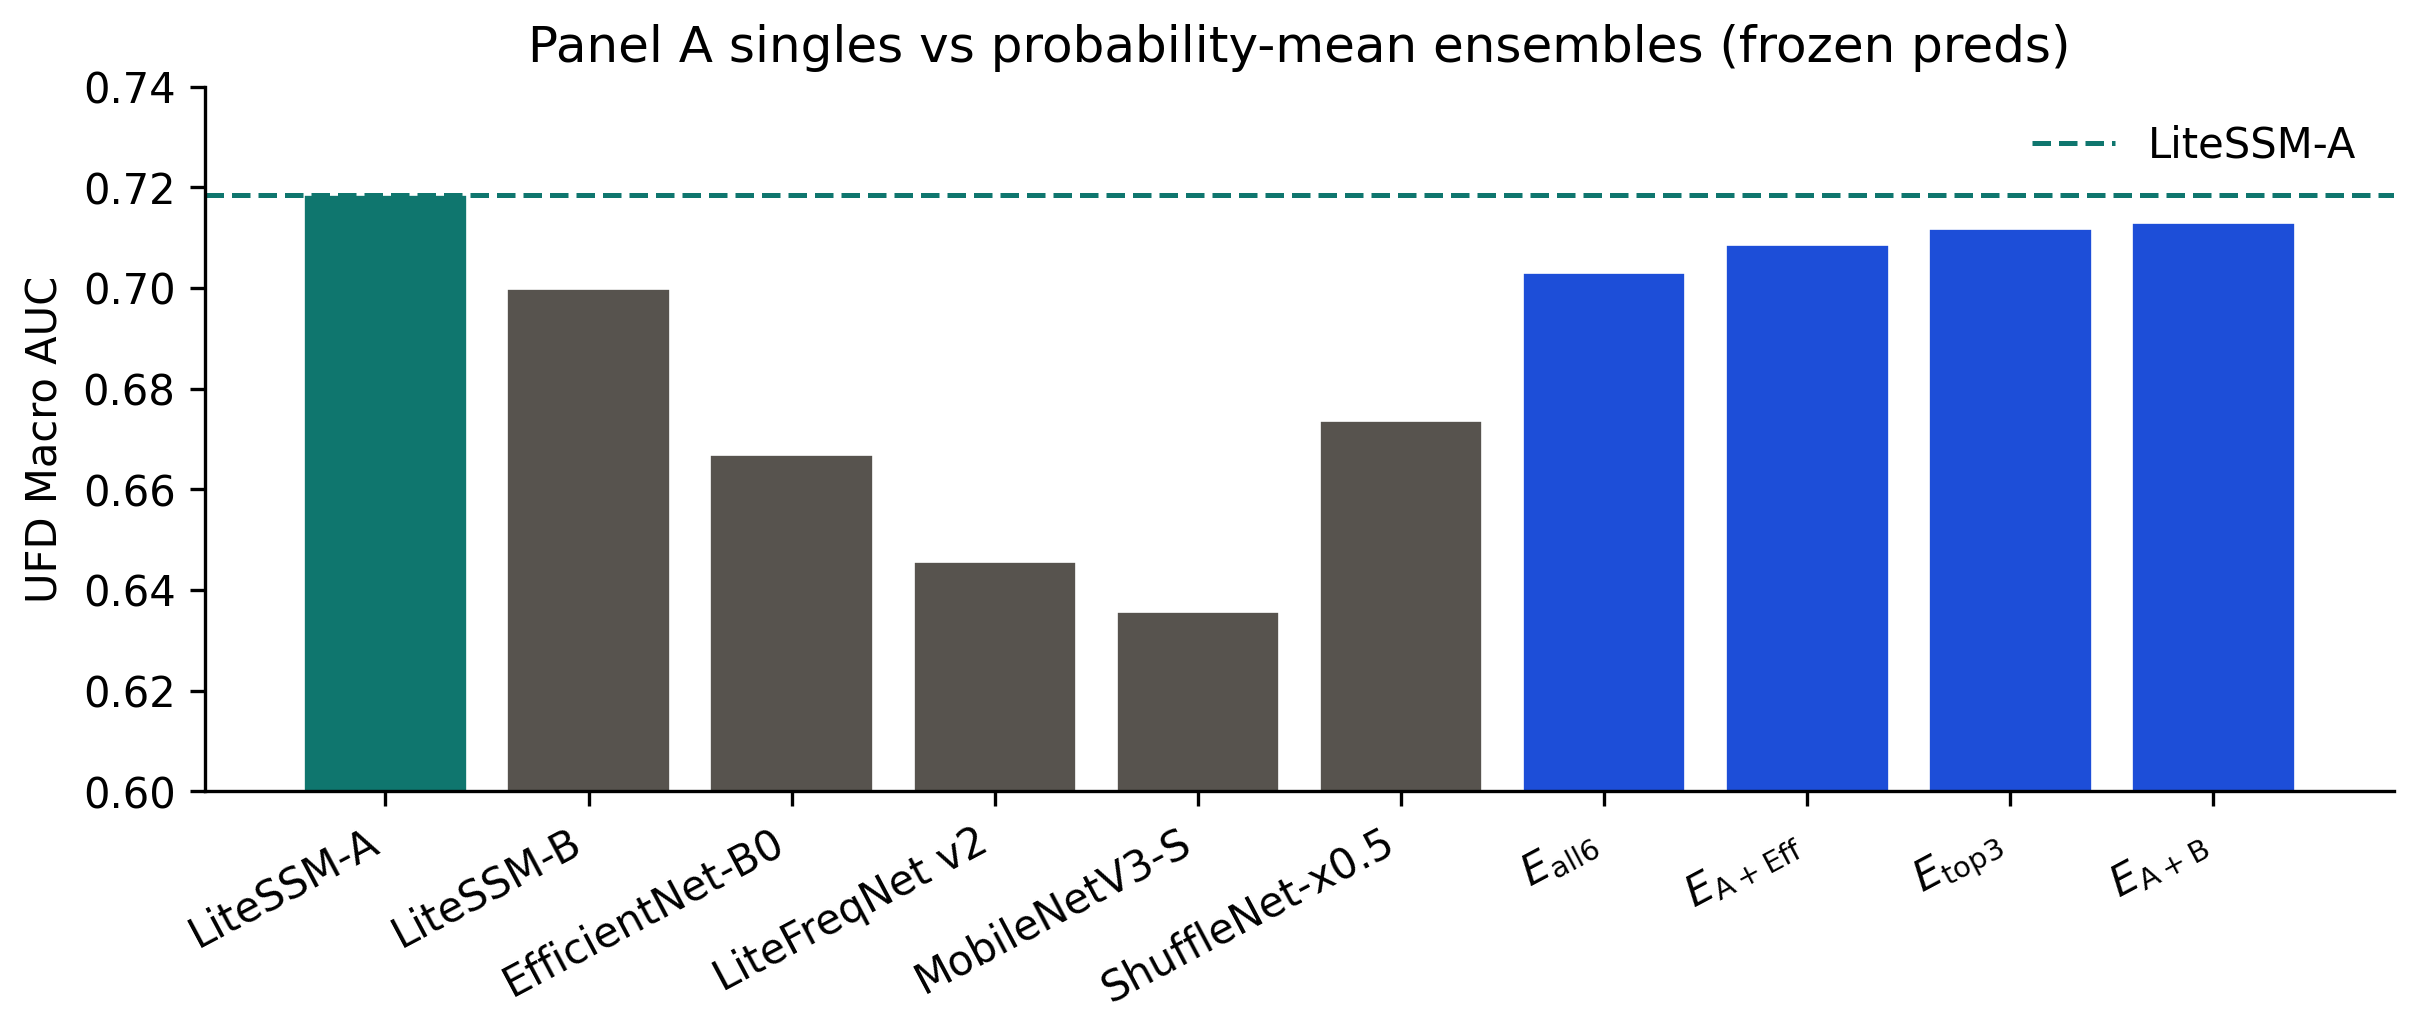
\includegraphics[width=0.92\textwidth]{figures/fig_ensemble_ufd_macro.png}
\caption{UFD Macro AUC for Panel~A singles and probability-mean ensembles computed from frozen prediction files.
No ensemble exceeds LiteSSM-A (dashed teal).\label{fig:ensemble}}
\end{figure}

\noindent\textbf{Reading.}
No probability-mean ensemble exceeds LiteSSM-A on UFD Macro (best ensemble Macro $0.713$ vs.\ $0.718$).
$E_{\mathrm{A+Eff}}$ raises DALL·E/Worst to $0.524$ but still loses Macro, confirming that averaging complementary singles does not automatically repair generator-macro collapse.
Double-fault rates versus LiteSSM-A on UFD remain substantial (e.g., error Jaccard $\approx$0.55--0.70 with other Panel~A models in \texttt{docs/ensemble\_panel\_a.json}), consistent with Appendix~\ref{app:diagnostics} $\kappa$ heatmaps: many failures are shared protocol-level blind spots rather than orthogonal errors that ensembles can cancel.

\subsection{Exploratory Matched-Generator Adaptation (Post-Freeze Probe)}
\label{app:m1v2}

After locking the Panel~A protocol, we ran an exploratory matched-generator adaptation probe (M1/M1-v2) outside the paper freeze: CE training on modern FLUX/SDXL images with an ID-anchor KL term, selected by \texttt{fixed\_last} without UFD hyperparameter search.
Table~\ref{tab:m1v2-app} summarizes descriptive AUCs.

\begin{table}[H]
\caption{Exploratory matched-generator adaptation (not a Panel~A main-table method; selection forbidden on UFD and on held-out SD3.5).\label{tab:m1v2-app}}
\scriptsize
\setlength{\tabcolsep}{3.5pt}
\begin{tabularx}{\textwidth}{@{}L*{5}{R}@{}}
\toprule
\textbf{Run} & \textbf{ID} & \textbf{UFD Macro} & \textbf{DALL·E} & \textbf{Held-out SD3.5} \\
\midrule
LiteSSM-A (baseline) & 0.946 & 0.718 & 0.504 & 0.694 \\
M1 (Phase-0 CE+anchor) & 0.936 & 0.652 & 0.410 & --- \\
M1-v2 (FLUX+SDXL train) & 0.933 & 0.683 & 0.444 & 0.844 \\
\bottomrule
\end{tabularx}
\end{table}

Matched-generator adaptation improved descriptive performance on a held-out SD3.5 probe ($0.694\rightarrow0.844$) and partially recovered M1's Macro regression ($0.652\rightarrow0.683$), yet UFD Macro and DALL·E remained below the baseline.
We therefore treat M1-v2 as \textbf{domain-specialization evidence}, not as a main-table positive method: target-family adaptation must not be conflated with broad cross-generator generalization.
No learning-rate, mix-ratio, or loss-weight sweeps were performed on SD3.5 or UFD for this probe.
